\documentclass[12pt, wide]{mwart}
\usepackage[utf8]{inputenc}  
\usepackage[english]{babel}
\usepackage{graphicx}    
\usepackage{epstopdf}
\usepackage{amsmath,amssymb,amsfonts,amsthm,mathtools}
\usepackage{xcolor}
\usepackage{bbm}  
\usepackage{hyperref}
\usepackage{url}
\usepackage{algorithmic}
\usepackage{float}
\usepackage{array}
\usepackage{algorithm}
\usepackage{braket, booktabs}
\setlength\extrarowheight{3pt}

\DeclareMathOperator*{\argmax}{arg\,max}
\newtheorem{lem}{Lemma}

\usepackage{afterpage}

\newcommand\blankpage{%
    \null
    \thispagestyle{empty}%
    \newpage}


\begin{document}
\newpage
\thispagestyle{empty}
\begin{center}
\textbf{\large University of Wrocław \\Faculty of Mathematics and Computer Science\\ Institute of Computer Science}\\
\textit{\large  Computer Science}\\
\vspace{4cm}
\textbf{\textit{\large Stanisław Wilczyński}\\
\vspace{0.5cm}
{\Large Microarray data analysis in prediction of breast cancer metastasis}}\\
\end{center}
\vspace{3cm}
\begin{center}

\large {Master thesis\\
under supervision of\\
Professor Jan Chorowski\\}

\end{center}

\vfill
\begin{center}
\large Wrocław 2019\\
\end{center}

\afterpage{\blankpage}
\newpage
\tableofcontents    
\section{Introduction}

\subsection{Overview}
One of the major problems of modern medical studies is the prediction of future metastases of breast cancer diagnosed patients. Although metastases are the main cause of death of such patients and despite the effort in uncovering the underlying mechanism, there was only a minimal improvement in the field in recent years. The main concern is the lack of reliable method to classify patients to 'poor prognosis' and 'good prognosis' groups. The first one refers to patients that would develop a distant metastasis within five years sine first tumor appearance. According to \cite{Metastasis1} the mechanism of distinguishing between these two classes could greatly reduce the number of patients unnecessarily receiving chemotherapy. Data mining seems to be a great candidate for automating the process of such diagnosis as it could allow to predict the outcome of the disease based on hidden, almost impossible to detect correlations or dependencies within the data. One of the most appealing candidate for highly informative data is the level of gene expression collected from the tumor cells. There are numerous examples of such data proving to be useful in tumor classification (\cite{BreastCancerClassification}, \cite{TumorMolecularClass}, \cite{TumorsClass1}, \cite{TumorClass2}). Unfortunately, the analysis of gene expression can be problematic, due to the number of features (measurements of expressed genes) being much higher than the number of samples (patients), as the extraction of gene expression data is costly. Such relation causes a phenomenon called 'curse of dimensionality' (\cite[p. 22-26]{ESL2}). In order to decrease this effect the dimensionality reduction techniques are often applied (\cite{MasterArts}, \cite{TumorClass4}, \cite{TumorPLS}). Such reduction even allows to use with success one of the most popular and state-of-the-art techniques such as neural network (\cite{fDNN}), which does not work in the settings where number of features is significantly higher than number of samples. Another important techniques are building a sparse representation (\cite{TumorClass3}) or using strong regularization (\cite[p. 649-666]{ESL2}) in constructed models. However, in scope of prediction of metastases data-mining methods are not so popular. In fact, current research focus mostly on purely biological markers (\cite{Metastasis4}, \cite{dataOrigin}), use prior knowledge based on protein-protein interaction networks (\cite{MetastasisScores}) or operate on very small samples (less than $100$ patients) and utilize only basic classification methods (\cite{Metastasis1}, \cite{Metastasis2}). Such reluctance to adopt more advanced models is usually caused by the requirement of having a model which can be easy to interpret. In terms of gene expression data it refers to being able to highlight the genes having the highest influence on the response. In this thesis, we focus on comparing different classification, dimensionality reduction or feature selection/extraction methods in order to find the ones applicable in the field of prediction of future metastases of breast cancer diagnosed patients. We use a gene expression data set consisting of $969$ patients for whom $12179$ genes expression levels were measured.

\subsection{Contribution}

In this thesis we present different classification and dimensionality reduction methods, discuss their advantages and weaknesses and apply them to the gene expression data. The main contribution is showing how this methods could help in providing automatic diagnosis and deciding about potential highly toxic treatment. Moreover, we show that previously used methods are outperformed by our framework. The code for all the experiments performed in this thesis is available at \url{github.com/sjwilczynski/geneExpr}.  

\subsection{Outline}
In section 2 we explain the medical notions in the simplified form to make it understandable for a person with very little biological knowledge and explain how our data set was collected and processed. In section 3 we discuss the methods used for classification and dimensionality reduction. In section 4 we statistically and graphically inspect our data. In section 5 we present the results of our analysis and discuss them. In section 6 we consider the medical applications and show how specific requirements in the field implies some tuning of our models. In section 7 conclusions are presented.

\section{Gene expression data}

\subsection{Biological background} \label{section:bio}
In this section we briefly explain biological notions used throughout the thesis, based on \cite{NHGRI} and \cite[chapters~11,12]{GeneExpr}. The \textit{cell} is the smallest structural and functional unit of a living organism that is able to run a biological processes (e.g metabolism, growth, reproduction). Every cell contains a \textit{DNA} (deoxyribonucleic acid) which is a chemical compound carrying the information needed to develop and direct the activities of the cell. DNA is composed two chains coiling around each other, which are made of four basic chemical units called nucleotides. A \textit{DNA sequence} is a particular arrangement of these nucleotides within a chain. This arrangement is what codes a unique characteristic of an organism. A \textit{genome} is an entire DNA sequence of a living creature. A \textit{gene} refers to a specific fragment of genome that has a distinct purpose, especially carries instructions for producing a protein. \textit{Proteins} are basic functional molecules in organisms, that among many applications within a cell control chemical reactions, regulate growth and participate in communication in biological pathways. In case of DNA mutation, the information it contains can be corrupted, causing a production of undesirable protein and disruption of standard flow of biological process. Such disruption, if undetected by immunological system can lead to development of diseases.

\textit{Gene expression} is the process during which the instructions coded in gene are used to synthesize its product. The level of expression corresponds to the amount of molecules created during this process. The gene is \textit{upregulated} if it synthesizes more, and \textit{downregulated} if synthesizes less when compared with such production in some reference conditions, assumed to be a homeostasis. The state-of-the-art technique for measuring relative expression levels is gene expression profiling using DNA microarrays. The main application of microarrays is to discover how genes functioning changes in response to genetic and environmental variations. \textit{Microarray} is a glass or plastic surface with microscopic spots, placed in regular intervals. Each spot contains picomoles ($10^{-12}$ moles) of a specific DNA sequence, known as \textit{probes}. Probes react with final or \textcolor{blue}{TODO nie finalny} results of gene expression process. By using products from two different cells (e.g cancer and healthy) on the same microarray we can measure the ratio of expression. These ratios are later gathered to form a vector of expression ratios of different genes. In order to conduct a research aimed at specific disease we collect vectors for different individuals with common condition and form a matrix. This matrix is referred as \textit{gene expression data}. \textcolor{blue}{TODO - potrzebny backup - review tej czesci i referencja do ksiazki}. As stated in \cite{preprocessing} there are two main sources of variations in microarray measurements. The first one called \textit{interesting variation} corresponds to the case when, for example, highly upregulated gene causes an illness and there is a noticeable difference between diseased and normal tissue. However, the other one called \textit{obscured variation} is induced by differences in the process of sample preparation, microarray manufacturing or even collecting the results from an array. Due to such diversity of possible factors influencing the results obtained from a microaaray it is crucial to apply normalization methods before actual data analysis in order to avoid misleading or even completely incorrect conclusions.

A tumor is a mass formed by a group of abnormal cells. This abnormality refer to disruption in the process of division and apoptosis. However, not all tumors are cancerous. The cancerous tumors (referred as malignant) are characterized by uncontrolled growth and division that leads to damaging nearby tissues. The process of spreading cancerous cell from primary source to other parts of body is called metastasis. Simplifying, it can be described as partial detachment of the tumor its transport with blood to other part of the organism Such secondary pathological sites are called metastases and are particularly dangerous. The gene expression data is of great interest in cancer related research as the alteration of cancerous cell division pattern is usually caused by either a mutation in a set of genes or a change in expression level and in consequence amount of proteins produced. 

\subsection{Data description} \label{section:description}

The data set consists of $969$ patients. Each patient is represented by the array measurement of the expression level from his cancerous cell. Such measurement has its unique identifier (e.g \textit{GSM177885}) referring to Gene Expression Omnibus (\cite{GEO}, \cite{NCBI2}). Gene Expression Omnibus is public database storing various forms of high-throughput functional genomic data. The repository is maintained by US organization National Center for Biotechnology Information and the data is uploaded and reviewed by scientific community. The \textit{GSM} prefix indicates that this identifiers corresponds to a single sample/cell. Other prefixes refer to series of data gathered within the same conditions (\textit{GSE}), platform (specific micorarray technology) used to perform the experiment (\textit{GPL}), collections of samples assembled by GEO staff (\textit{GDS}). In case of our data set, it was assembled from 10 public microarray data sets, namely: GSE25066, GSE20685, GSE19615, GSE17907, GSE16446, GSE17705, GSE2603, GSE11121, GSE7390, GSE6532. Each series was obtained using Affymetrix Human Genome HG-U133 Plus 2.0 and HG-U133A arrays, which refer to the mentioned earlier platform. As explained in \ref{section:bio} it is essential to preprocess data before the analysis. Therefore, each data set was first normalized using quantile normalization described in \cite{quantileNorm}, then further processed using robust multi-array average (RMA) probe summary algorithm from \cite{preprocessing}. Due to the fact that these series could have different number of genes expression measured they were combined together on the basis of HG-U133A array probe names resulting in reducing the number of variables to $12179$. Each variable correspond to a level of expression of a specific gene (e.g. RPL41). Each patient is also labeled. Label $1$ corresponds to people who had metastatic event within 5 years from being cancer diagnosed. $0$ corresponds to people who had the first follow up after $5$ years or no metastasis at all. There are $393$ and $576$ samples with labels $1$ and $0$ respectively.

\section{High dimensional data analysis}

\subsection{Background and challenges} \label{section:challenges}

As stated in the introduction our aim is prediction of future metastases which in terms of our data translates to binary classification problem using the labels. There are numerous examples where classification methods allow to solve very complex problems e.g customer target marketing, document categorization and filtering or computer vision (\cite{dataClassification}). However, in the field of biomedical data not all of them are applicable in our setting. The reason is the high dimensional, complex structure of our data, particularly the relation between the number of samples and number of features: $n \ll p$. As mentioned in the section \ref{section:bio} such relation is caused by the relatively low availability of samples and high costs of extracting, processing and labeling new ones. These activities have to be done in laboratory by professionals, in comparison to creation of data sets containing images where anyone can participate in e.g paid labelling procedure. Apart from that huge number of features causes a phenomenon called \textit{curse of dimensionality}. As described in \cite{ISL} the increase in the number of variables can improve the model only if the added features are signals - associated with the response. On the other hand, if they do not influence the response at all, they introduce noise. This may lead to overfitting and significantly larger test error (more details in section \ref{section:selection}). The source of this problem is that with increasing dimension the sample space become very sparse and all pairwise distances between data points are alike. Furthermore, huge number of variables introduces more complexity in most models as the number of parameters to estimate grows. In extreme cases it may even lead to lack of convergence in parameter estimation and in consequence lack of model stability. In order to tackle this issue we will use robust classifiers and dimensionality reduction procedures described in further chapters.

\subsection{Classifiers for high dimensional data}

\subsubsection{Logistic regression and its modifications}

One of the most popular and simple classifiers for binary response is logistic regression (LR). It is a counterpart of linear regression for regression problems and was proven to be valuable method for microarray analysis (\cite{LRgene}). The model aims at estimating the conditional probability of class membership. It is described by the following formula:
\begin{align*}
    &P(y=1 | x, \beta)=\sigma\left(\beta^{T} x\right) \\
    &\sigma(t) = \frac{1}{1+e^{-t}} \\
    &x=(1, x_1, \ldots, x_p) \\
    &\beta = (\beta_0, \ldots, \beta_p)
\end{align*}
where $x$ is the vector of features, $\beta$ is the vector of coefficients including intercept, $\sigma$ is sigmoid function and is used to squeeze the output to range $(0,1)$ and P is the conditional probability of class $1$ a sample described by variables $x$. The interpretation of logistic regression coefficients is quite different than linear regression due to the usage of sigmoid function. In terms of the latter one an increase of one unit of variable $x_i$ corresponds to increase of the output by $\beta_i$. The similar relation for LR can be expressed using log odds (the ratio of probabilities of event occurring and not occurring):

\begin{align*}
    \log \left(\frac{P(y=1| x, \beta)}{1-P(y=1| x, \beta)}\right)=\log \left(\frac{P(y=1| x, \beta)}{P(y=0| x, \beta)}\right)=\beta_{0}+\beta_{1} x_{1}+\ldots+\beta_{p} x_{p}
\end{align*}

Above equation clearly indicates that an increase of one unit of variable $x_i$ corresponds to increase of the log odds by $\beta_i$ and this implies and increase of odds ratio by a factor of $\exp(\beta_i)$. Similarly $\beta_0$ corresponds to the log odds in the baseline conditions. Such relatively simple and probabilistic interpretation made the model very popular. However, it has some disadvantages. First of all, it does not incorporate a possibly complicated correlation structure or interactions between variables. Secondly, it could perform worse with highly correlated features or features having no influence on response and coefficients could be infinite in case of occurrence of complete separation, i.e when one feature can distinguish completely between classes. Nonetheless, LR is widely used, also due to uncomplicated learning scheme. Similarly to linear regression coefficients in LR are calculated using maximum likelihood estimation. The likelihood function takes the form:
\begin{align*}
    L(\beta) = \prod_{i=1}^n P(Y=y_i | x_i, \beta) &= \prod_{i=1}^n P(Y=1 | x_i ; \beta)^{y_i}(1-P(Y=1 | x_i ; \beta))^{\left(1-y_i\right)} \\
&= \prod_{i=1}^n \sigma\left(\beta^{T} x_i\right)^{y_i}\left(1-\sigma\left(\beta^{T} x_i\right)\right)^{\left(1-y_i\right)}
\end{align*}
And the negative log likelihood is:
\begin{align*}
    nll(\beta)=-\sum_{i=1}^{n} y_i \log \sigma\left(\beta^{T} x_i\right)+\left(1-y_i\right) \log \left(1-\sigma\left(\beta^{T} x_i\right)\right)
\end{align*}

In the two above equations $x_1, \ldots x_n$ denote samples and $y_i$ corresponding labels. In order to maximize the coefficients we calculate the first derivative of the negative log likelihood function as in \cite[chapter 4.4.1]{ESL2}:
\begin{align*}
    \frac{\partial nll(\beta)}{\partial \beta}&=\sum_{i=1}^{n}\left(\sigma\left(\beta^{T} x_i\right)-y_i\right) x_i\\ &=
    \left[\left(\sigma(X\beta) - Y\right)^TX\right]^T
\end{align*}
We can clearly see that the right side is not linear in $\beta$ and in fact equation $\frac{\partial nll(\beta)}{\partial \beta} = 0$ cannot be solved analytically. Therefore, the maximizing coefficients are found using Newton-Raphson method, extensions of gradient descent like SAG (\cite{sag}) or SAGA (\cite{saga}) and other e.g. Liblinear (\cite{liblinear}). 

However, classic logistic regression has one more drawback. Without any constraints in order to fit $p+1$ we need at least $p+1$, otherwise there are infinitely many solutions. For our data set $n \ll p$ and LR cannot work in such settings. Therefore, additional restriction is introduced to our model which is regularization. 



%Remember to discuss why LR doesn't work in the setting where $n << p$. \textcolor{blue}{\href{https://stats.stackexchange.com/questions/139353/why-does-logistic-regression-not-work-in-p-n-setting}{link}}

L1 and L2 - its connection with prior distributions (as in PGM)

\subsubsection{Linear Discriminant Analysis and Nearest Shrunken Centroid}

\subsubsection{Linear Support Vector Machines}

\subsubsection{Ensemble models}

Random forest, random logistic regressions


\subsection{Dimensionality reduction}

\subsubsection{PCA and SPCA}

\subsubsection{Partial Least Squared}

\subsubsection{Forest Deep Neural Network}

\subsubsection{Multiple Latent Components Clustering}


\subsection{Model assessment and selection} \label{section:selection}

Good section in ESLII


\begin{itemize}
    \item train, val, test split discussion 
    \item choice of hyperparams and cross validation
    \item ROC
    \item Preference of recall over ROC  - maybe move to applications section
    \item Confusion matrix(?)
\end{itemize}


\section{Exploratory analysis}

In this section we present the results of exploratory analysis. Although preprocessing has already been applied, such analysis should be performed to get a deeper understanding of the data. It involves analyzing main statistical characteristics, study of missing values and outliers, visualization, feature removal and normalization. Due to earlier preprocessing (quantile normalization and RMA introduced in \ref{section:description}), we expect our variables to follow normal distribution. To assess accuracy of this statements we plot values of four common statistics: mean, standard deviation, skewnees and kurtosis. Skewness measures the asymmetry of the distribution and is equal to the third standardized moment, whereas kurtosis corresponds to the heaviness of the tails of the distribution and is equal to fourth standardized moment. High kurtosis indicates heavy tails or outliers when calculated from sample. For normal distribution skewness and kurtosis are $0$ and $3$ respectively. Below are the mathematical formulas for these statistics:
\begin{align}
    Skew[X] = E\left[\left(\frac{X-\mu}{\sigma}\right)^3 \right] \nonumber \\
    Kurt[X] = E\left[\left(\frac{X-\mu}{\sigma}\right)^4 \right] \nonumber
\end{align}
In the code we use \textit{scipy.stats.kurtosis} to calculate the kurtosis which subtracts $3$ from the result to make $0$ the value for normal distribution. 

\begin{figure}
\centering
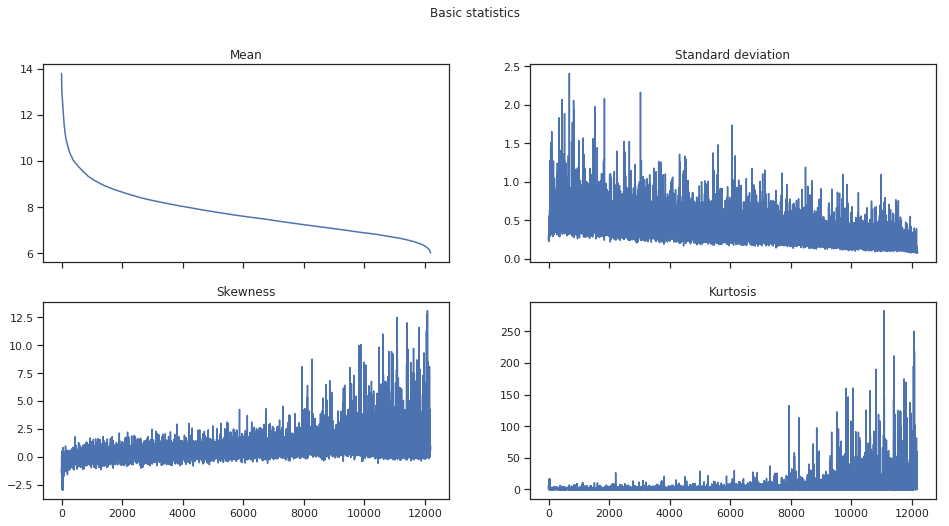
\includegraphics[width=\textwidth]{images/basic_stats.png}
\caption{Main statistical characteristics of the data}
\label{fig:stats}
\end{figure}

On the figure \ref{fig:stats} we can see that the data is not standardized. The variables are sorted decreasingly by means varying from $6.01$ to $13.79$. Also standard deviations vary from $0.07$ to $2.41$. Therefore, before applying any dimensionality reduction method we should standardize our data, e.g in PCA the variance explained by a variable hugely depends on its scale and could lack of standardization could lead to over or underestimation of its effect. Skewness and kurtosis evidence against our normality assumption. They vary from $-2.99$ to $13.10$ and $-1.38$ to $282.88$ respectively. Especially, the kurtosis implies presence of outliers. In order to get more insight on the distribution of our variables in figure \ref{fig:hists_out} we plot the histogram and boxplots of genes with maximum skewness and kurtosis and in figure \ref{fig:hists_norm} we plot histograms and boxplots of randomly chosen genes from the data. 

\begin{figure}
\centering
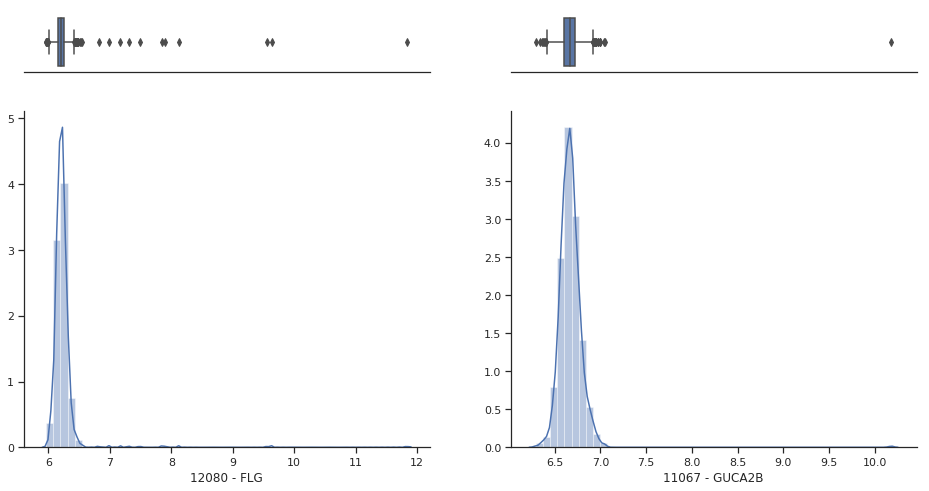
\includegraphics[width=\textwidth]{images/hists_ouliers.png}
\caption{Histograms of genes with maximum skewness and kurtosis}
\label{fig:hists_out}
\end{figure}

\begin{figure}
\centering
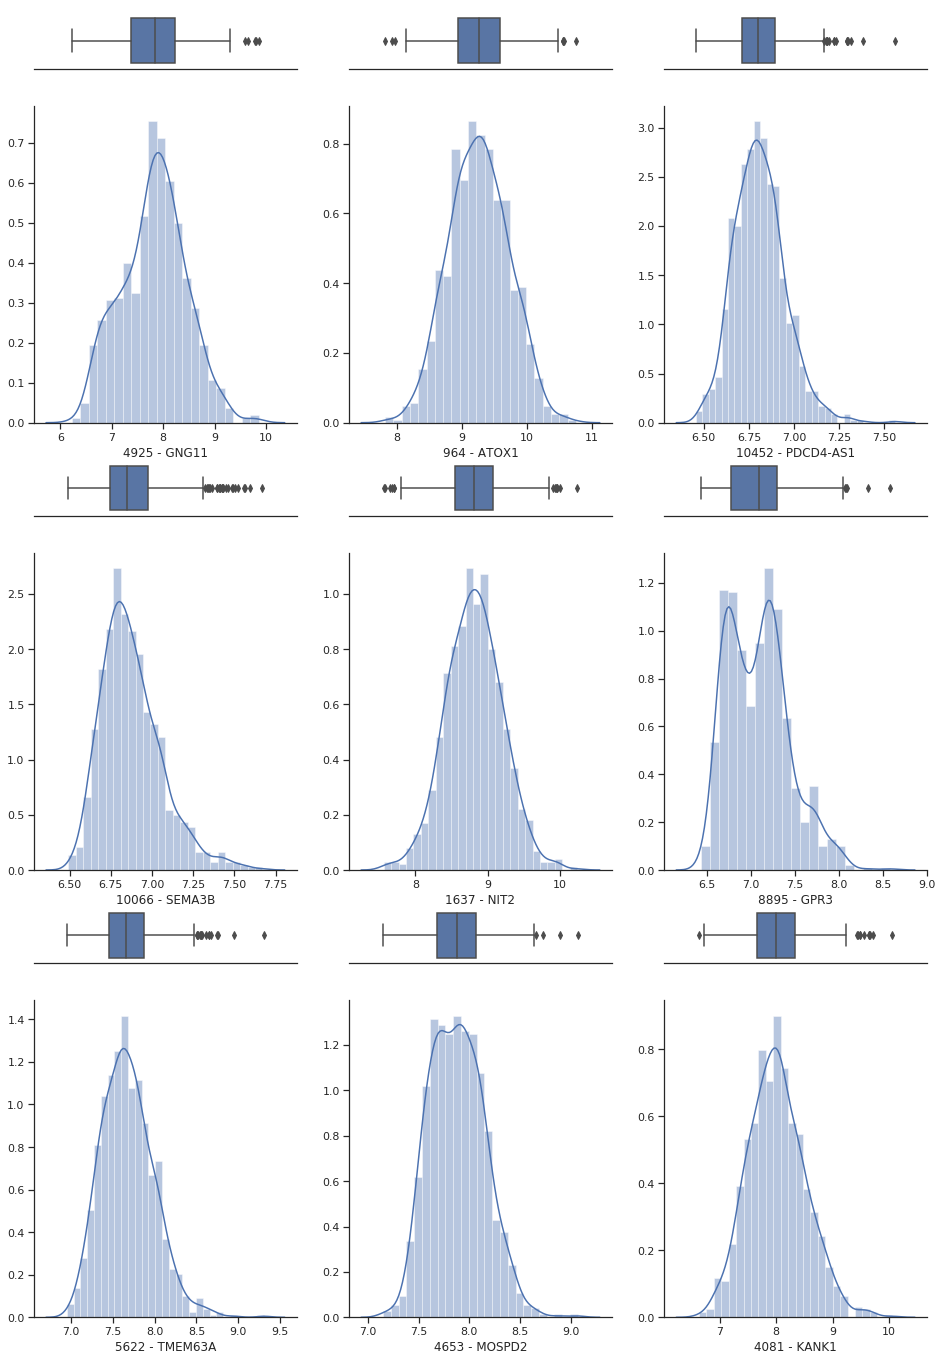
\includegraphics[width=0.95\textwidth]{images/hists_normal.png}
\caption{Histograms of randomly chosen genes from the data}
\label{fig:hists_norm}
\end{figure}


By looking at the figure \ref{fig:hists_norm} we conclude that also the distribution are visibly skewed and even multimodal they do not indicate that further transformation is needed to able to use models assuming normality. However, we can clearly see form figure \ref{fig:hists_out} that high skewness or kurtosis can be caused by outlying values for this variable. In order to verify this we calculate the 95\% quantile for both skewness and kurtosis. They are equal to $2.15$ and $9.77$ respectively. It indicates that only very few genes have statistics indicating strong non normality. What is more, the number of genes with kurtosis or skewness above 95\% quantile is $710$ which is not significantly larger than the number of genes with high kurtosis only. This indicates that the extreme values of either of these statistics appear on the small subset of genes. In order to assess the influence of such genes we consider following data sets: data set consisting of genes only with values of skewness and kurtosis below the 95\% quantile ($D_1$), the complement of the previous data set ($D_2$), $50$ data sets extracted by randomly choosing $710$ variables from the original data ($D_{random}$). We split each of them to train and test parts and fit logistic regression with L1 penalty and regularization hyperparameter chosen using cross validation as described in section \ref{section:selection}. We compare the scores on the test set (section \ref{section:selection}) to check how these genes with outlying values impact our prediction. For the random data sets we fit the model for each of them and take the mean scores. The results are presented in the table \ref{tab:scores-trunc}: 
\begin{table}[H]
\centering
    \begin{tabular}[t]{c c c c c}
    \toprule
    & ROC AUC & Precision & Recall & F1\\
    \midrule
    $D_1$ & $0.827$ & $0.718$ &	$0.712$ & $0.715$ \\
    $D_2$ & $0.742$ & $0.659$ & $0.577$ & $0.615$ \\
    $D_{random}$ & $0.787$ & $0.700$ & $0.616$ & $0.655$ \\
    \bottomrule
\end{tabular}
    \caption{Scores of logistic regression with subsets of variables}
    \label{tab:scores-trunc}
\end{table}

From this table we can clearly see that the genes in $D_2$ do not have big predictive power. The mean scores from $D_{random}$ are higher for every considered metric. It is also worth noting that randomly chosen variables bring less information for prediction than all the genes in $D_1$. The next step is checking how these genes with extreme values impact stability of our classifier.

In order to check it we use six different transformations on the data, then fit logistic regression model with L1 penalty and the same regularization parameter. We choose this classifier because its weights are sensitive to outliers and could easily indicate the impact of genes with extreme values. 
The compared transformations are:

\begin{enumerate}
    \item No transformation
    \item Standardization - from each variable we subtract its mean and divide by standard deviation
    \item Quantile transformation to normal distribution - for each variable we calculate the empirical cumulative density function (CDF) and use it to project original data. The projected data is truncated to $10^{-7}$ and $1-10^{-7}$ then transformed using inverse CDF of normal distribution. The formula is $y_{i}=\Phi^{-1}\left(F\left(x_{i}\right)\right),$ where $F$ and $\Phi$ represent empirical CDF and normal distribution CDF respectively. This transformation is more robust to outliers than scaling but may deform distances within and across features.
    \item Quantile transformation to uniform distribution - similar to the previous one but we transform data to match uniform distribution. We use it to check how the weights of logistic regression will be affected when unreasonable transformation is applied to our data.
    \item Truncating most extreme values - for each feature we calculate 1\% ($q_1$) and 99\% ($q_{99}$) quantiles and replace values smaller then $q_1$ with $q_1$ and values greater then $q_{99}$ with $q_{99}$
    \item Quartile standardization - for each variable we subtract its median and divide by inter quartile range which is equal to difference between 75\% quantile and 25\% quantile
\end{enumerate}

\begin{figure}
\centering
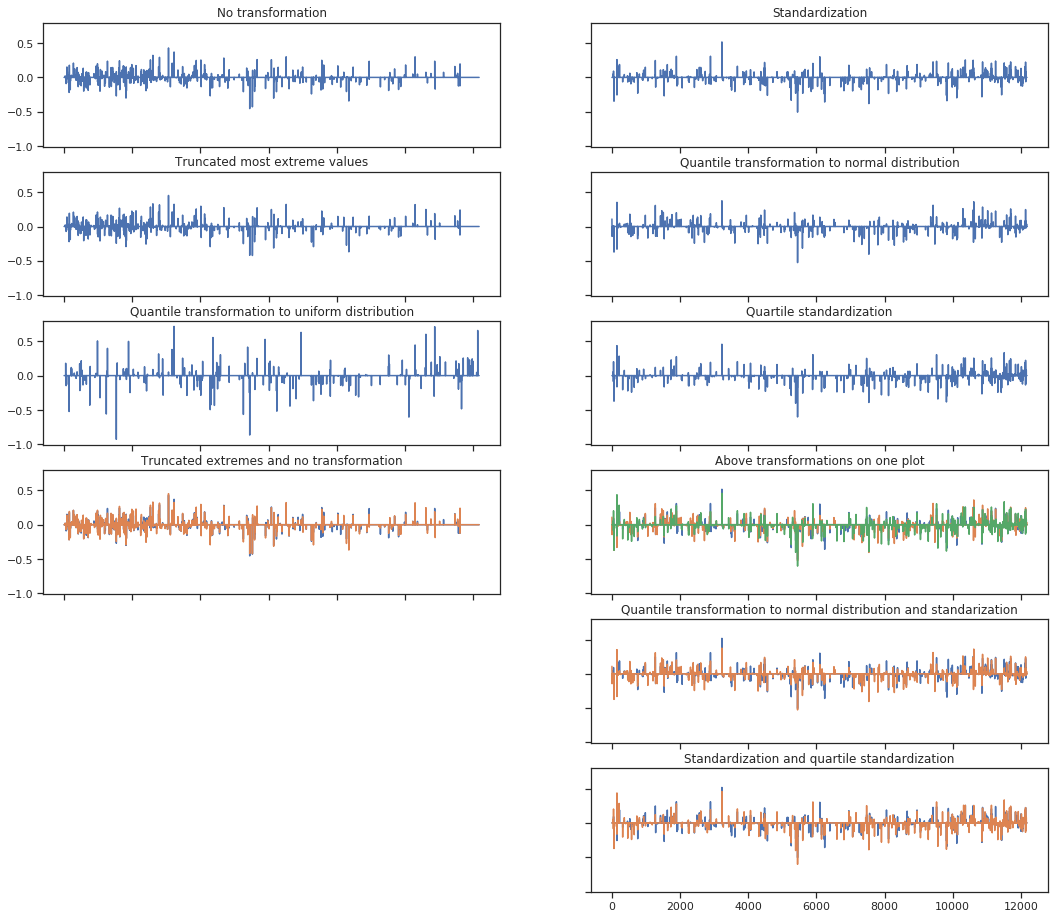
\includegraphics[width=\textwidth]{images/normalization_coeffs.png}
\caption{Weights of logistic regression with different data transformations}
\label{fig:normalization}
\end{figure}

The plots of the weights of these classifiers are presented on figure \ref{fig:normalization}. We can see that the difference between no transformation and truncating extreme ($4$-th plot in the first column) values is very small. It indicates that these genes with very high skewness and kurtosis do not impact our prediction significantly and do not need to be truncated or removed from the data. What is more application of different transformation aiming to normalize our features (plots $4-6$-th in the second column) resulted in similar logistic regression coefficients. Taking into account figure \ref{fig:hists_norm} and \ref{fig:normalization} we conclude that there is no justification of using other transformation of our data set before further analysis. We will only standardize the data before applying dimensionality reduction methods as they are sensitive to features' scales.

In data mining we usually aim to remove strongly correlated variables from the data, due to the possibility of causing instability in our models (\cite{Correlation}). In case of gene expression data this usually refers to genes which are co-regulated and involved in the same genetic pathway. In order to get notion of such correlation structure we present (figure \ref{fig:heatmap}) the correlation between randomly chosen $50$ genes. 

\begin{figure}
\centering
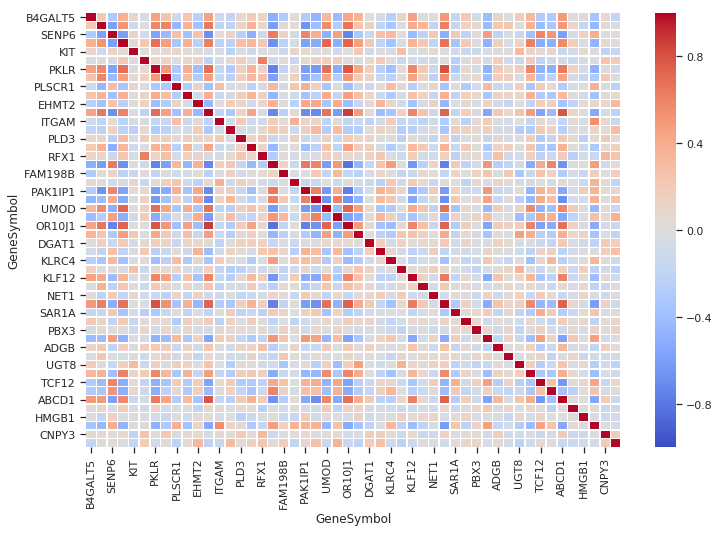
\includegraphics[width=0.8\textwidth]{images/heatmap.png}
\caption{Correlation of randomly chosen subset of $50$ genes}
\label{fig:heatmap}
\end{figure}

Although most variables seem to have correlation close to $0$ we can clearly see some significant ones, even though we chosen randomly only $0.41$\% of our variables. This correlation matrix strongly indicates that dimensionality reduction methods (both feature selection and extraction) can be exploited on our data.

\section{Results}

\begin{itemize}
    \item Something about code - used libraries, computational power, implementations etc.
    \item Best models - present ROC curves, adjust errors from ROC, some explanation, comparison with model chosen by recall
    \item comparison with other papers - e.g. most popular classification based on 76 selected genes
\end{itemize}


\section{Applications in medicine}

\begin{itemize}
    \item What is acceptable in medicine
    \item Not liking black box models, Linear vs nonlinear
    \item Feature extraction vs feature selection
    \item pathway enrichment
\end{itemize}

\section{Conclusion}

\bibliography{biblio}
\bibliographystyle{plain}
%\bibliographystyle{apalike}


\end{document}
